% *********************************************************************
% © 2021–2026 Jeremy Sylvestre
%
% Permission is granted to copy, distribute and/or modify this document
% under the terms of the GNU Free Documentation License, Version 1.3 or
% any later version published by the Free Software Foundation; with no
% Invariant Sections, no Front-Cover Texts, and no Back-Cover Texts. A
% copy of the license is included in the appendix entitled “GNU Free
% Documentation License” that appears in the output document of this
% PreTeXt source code. All trademarks™ are the registered® marks of
% their respective owners.
%
% *********************************************************************

\newcommand*{\xmin}{-6.25}
\newcommand*{\xmax}{10.25}
\newcommand*{\ymin}{-1.5}
\newcommand*{\ymax}{1.5}

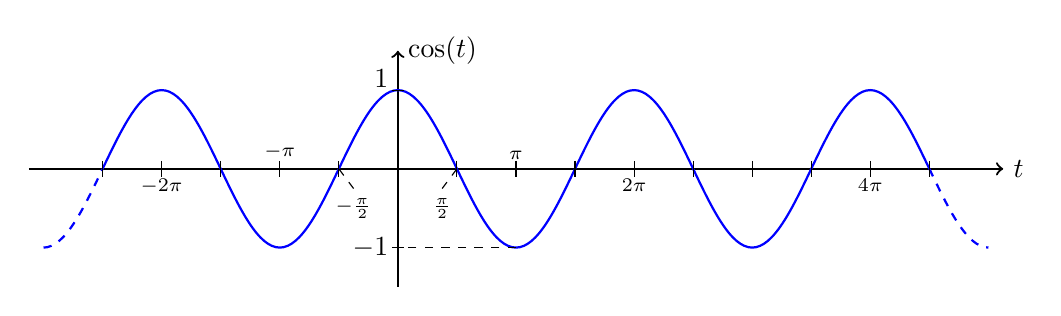
\begin{tikzpicture}
[
	closedpt/.style={circle,draw,fill,inner sep=0pt,minimum size=4pt},
	openpt/.style={circle,draw,inner sep=0pt,minimum size=4pt},
	xscale=0.75
]

	% axes
	\draw[->,thick] (\xmin,0) -- (\xmax,0) node[right] {$t$};
	\draw[->,thick] (0,\ymin) -- (0,\ymax) node[right] {$\cos(t)$};

	\draw[blue,thick,dashed] (-6,-1) cos (-5,0);
	\draw[blue,thick,dashed] (9,0) sin (10,-1);

	\draw[blue,thick]
	  (-5,0)
	  sin (-4,1)
	  cos (-3,0)
	  sin (-2,-1)
	  cos (-1,0)
	  sin (0,1)
	  cos (1,0)
	  sin (2,-1)
	  cos (3,0)
	  sin (4,1)
	  cos (5,0)
	  sin (6,-1)
	  cos (7,0)
	  sin (8,1)
	  cos (9,0)
	;

	\foreach \x in {-5,-4,-3,...,9} {
		\draw (\x,0.1) -- (\x,-0.1);
	}

	\node[below] at (-4,0) {$\scriptstyle -2 \pi$};
	\node[above] at (-2,0) {$\scriptstyle - \pi$};
	\draw[dashed] (-1,0) -- (-0.75,-0.25) node[below] {$\scriptstyle - \frac{\pi}{2}$};

	\draw[dashed] (1,0) -- (0.75,-0.25) node[below] {$\scriptstyle \frac{\pi}{2}$};
	\node[above] at (2,0) {$\scriptstyle \pi$};
	\node[below] at (4,0) {$\scriptstyle 2 \pi$};
	\node[below] at (8,0) {$\scriptstyle 4 \pi$};

	\node[left,yshift=0.15cm] at (0,1) {$1$};
	\draw[dashed] (2,-1) -- (0,-1) node[left] {$-1$};
	\foreach \y in {-1,1} {
		\draw (-0.1,\y) -- (0.1,\y);
	}

\end{tikzpicture}
